% !TEX TS-program = pdflatex
% !TEX encoding = UTF-8 Unicode

% This is a simple template for a LaTeX document using the "article" class.
% See "book", "report", "letter" for other types of document.

\documentclass[11pt]{article} % use larger type; default would be 10pt

\usepackage[utf8]{inputenc} % set input encoding (not needed with XeLaTeX)

%%% Examples of Article customizations
% These packages are optional, depending whether you want the features they provide.
% See the LaTeX Companion or other references for full information.

%%% PAGE DIMENSIONS
\usepackage{geometry} % to change the page dimensions
\geometry{a4paper} % or letterpaper (US) or a5paper or....
% \geometry{margin=2in} % for example, change the margins to 2 inches all round
% \geometry{landscape} % set up the page for landscape
%   read geometry.pdf for detailed page layout information

\usepackage{graphicx} % support the \includegraphics command and options

% \usepackage[parfill]{parskip} % Activate to begin paragraphs with an empty line rather than an indent

%%% PACKAGES
\usepackage{booktabs} % for much better looking tables
\usepackage{array} % for better arrays (eg matrices) in maths
\usepackage{paralist} % very flexible & customisable lists (eg. enumerate/itemize, etc.)
\usepackage{verbatim} % adds environment for commenting out blocks of text & for better verbatim
\usepackage{subfig} % make it possible to include more than one captioned figure/table in a single float
\usepackage[frenchb]{babel}
\usepackage[T1]{fontenc}
\usepackage{natbib,bibentry}
\usepackage{color}
\usepackage{listings}
\usepackage{yfonts}
\usepackage{epsfig}
\usepackage{amsmath,amssymb,amsfonts,calligra}
\usepackage{calc}
\usepackage{import}
\usepackage{hyperref}
\usepackage[utf8]{inputenc}
% \usepackage{tabto}
\DeclareGraphicsExtensions{.eps, .jpg, .png}
\DeclareMathOperator*{\argmin}{argmin}
% These packages are all incorporated in the memoir class to one degree or another...

%%% HEADERS & FOOTERS
\usepackage{fancyhdr} % This should be set AFTER setting up the page geometry
\pagestyle{fancy} % options: empty , plain , fancy
\renewcommand{\headrulewidth}{0pt} % customise the layout...
\lhead{}\chead{}\rhead{}
\lfoot{}\cfoot{\thepage}\rfoot{}

%%% SECTION TITLE APPEARANCE
\usepackage{sectsty}
\allsectionsfont{\sffamily\mdseries\upshape} % (See the fntguide.pdf for font help)
% (This matches ConTeXt defaults)

%%% ToC (table of contents) APPEARANCE
\usepackage[nottoc,notlof,notlot]{tocbibind} % Put the bibliography in the ToC
\usepackage[titles,subfigure]{tocloft} % Alter the style of the Table of Contents
\renewcommand{\cftsecfont}{\rmfamily\mdseries\upshape}
\renewcommand{\cftsecpagefont}{\rmfamily\mdseries\upshape} % No bold!
\parindent = 0mm
\bibliographystyle{plain}
\hoffset = -10mm
\voffset = -15mm
\textwidth = 165mm
\textheight = 240mm
\definecolor{lightgray}{gray}{0.2}
\definecolor{mygreen}{RGB}{28,172,0}
\definecolor{mylilas}{RGB}{170,55,241}
\newcommand{\expect}{{\rm I \mkern-2.5mu \nonscript\mkern-.5mu E}}
\newcommand{\equaldef}{\stackrel{d}{=}}
\newcommand{\argmax}{\operatornamewithlimits{argmax}}
\newcommand{\debutrep}[1]{\color{blue}\begin{center} \hrulefill \textbf{ #1 } \hrulefill \end{center} }
\newcommand{\finrep}{\vspace*{5mm}\hfill $\square$\color{black}\vspace*{5mm}}
\newcommand \tab[1][1cm]{\hspace*{#1}}
\newcommand{\G}{\text{\calligra G}\,}

%%% END Article customizations

%%% The "real" document content comes below...

\title{Analyse Numérique\\Equations Différentielles Ordinaires\\Mouvement keplérien et double pendule}
\author{Axel Bruyere, Dorian Fabregue\\4ETI-IMI}
%\date{} % Activate to display a given date or no date (if empty),
         % otherwise the current date is printed 

\begin{document}

\lstset{language=Matlab,%
    %basicstyle=\color{red},
    breaklines=true,%
    morekeywords={matlab2tikz},
    keywordstyle=\color{blue},%
    morekeywords=[2]{1}, keywordstyle=[2]{\color{black}},
    identifierstyle=\color{black},%
    stringstyle=\color{mylilas},
    commentstyle=\color{mygreen},%
    showstringspaces=false,%without this there will be a symbol in the places where there is a space
    numbers=left,%
    numberstyle={\tiny \color{black}},% size of the numbers
    numbersep=9pt, % this defines how far the numbers are from the text
    emph=[1]{for,end,break},emphstyle=[1]\color{red}, %some words to emphasise
    %emph=[2]{word1,word2}, emphstyle=[2]{style},    
}

\maketitle

\vspace*{15mm}
{\Large\bf Objectifs}~--~~\begin{minipage}[t]{135mm}
• Compréhension des EDO d'ordre 1 (Problème de Cauchy)\\
• Implémentation des méthodes d'Euler et de Runge-Kutta (ordre 2 et 4)\\
• Application de ces méthodes à l'étude du mouvement képlerien et du double pendule\\
• Compréhension des défauts de ces méthodes pour chaque étude\\
• Implémentation de nouveaux algorithmes afin d'améliorer les résultats de l'analyse numérique\\
\end{minipage}
\vspace*{10mm}

\section{Contexte}
Les équations différentielles ordinaires (EDO) interviennent dans de nombreux domaines de la modélisation mathématique. Nous allons nous intéresser ici en particulier à deux modèles mécaniques particuliers, à savoir:\\
\tab - Etude du mouvement képlerien (trajectoire d'un satellite orbitant autour d'un astre)\\
\tab - Etude du mouvement d'un double pendule non-amorti\\\\
Ces cas-là sont malheureusement trop complexes pour être résolus par des méthodes analytiques car ces situations sont modélisées par des systèmes d'équations différentielles non linéaires et ne présentent pas de solutions exactes.\\\\
Pour résoudre ces systèmes d'équations, nous allons mettre en place différents modèles de résolution, à savoir la méthode d'Euler et la méthode de Runge-Kutta (ordres 2 et 4). Nous analyserons les caractéristiques de chacun de ces modèles et mettrons en place, si possible, un nouveau modèle de résolution plus performant.


\clearpage

\tableofcontents
\clearpage
\section{Etude du mouvement képlerien}
\vspace*{5mm}

\subsection{Introduction}

En astronomie, plus précisément en mécanique céleste, le mouvement képlérien correspond à une description du mouvement d'un astre par rapport à un autre respectant les trois lois de Kepler (1571-1630). La première de ces trois lois, la "loi des orbites", énonce que les objets célestes gravitant autour d'une étoile décrivent des trjactoires elliptiques. C'est ce type de mouvement que nous allons essayer de modéliser dans cette partie.\\

Dans notre cas, nous supposons l’orbite elliptique avec une forte excentricité. Cela signifie que la distance entre la planète et l’étoile varie fortement entre l’aphélie (point le plus éloigné du l’étoile) et le périhélie (point le plus proche).  Dans ce cas, le mouvement de la planète $P=(x(t),y(t))$ est modélisé par le système d'équations différentielles suivant:
\begin{equation}
 \begin{cases} x''(t) +  \G M \dfrac{x(t)}{[x(t)^2+y(t)^2]^{3/2}} = 0\\ y''(t) +  \G M \dfrac{y(t)}{[y(t)^2+y(t)^2]^{3/2}} = 0\end{cases}
\end{equation}
où \G. est la constante de gravitation universelle, elle apparait dans la troisième loi de Kepler : 
\begin{equation}
\frac{a^3}{T^2}=\dfrac{\G M}{4\pi^2}
\end{equation}
où $a$ est le demi-grand axe de l’orbite elliptique et $T$ est la période de révolution de la planète autour de l’étoile.
\begin{figure}[h]
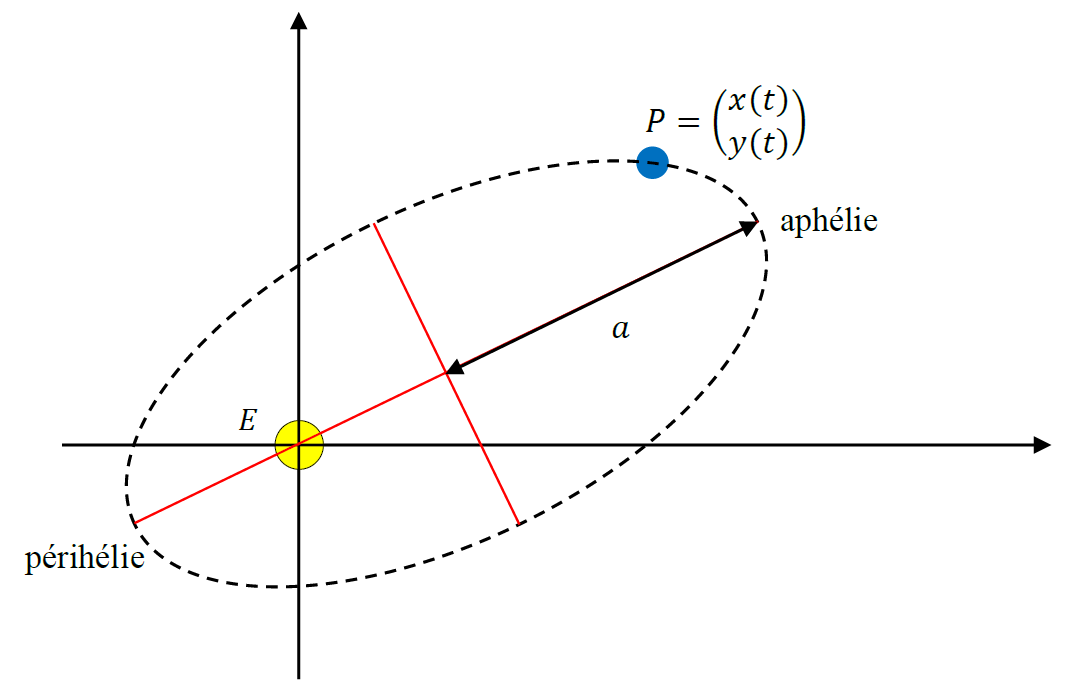
\includegraphics[width=10cm]{enonce_exo6}
\centering
\caption{Orbite elliptique (avec forte excentricité) d’une planète P autour d’une étoile E}
\end{figure}\\\\
Afin de résoudre ce système d'équations différentielles, nous allons mettre en place un programme utlisant différentes méthodes d'analyse numériques et essayer d'obtenir un résultat satisfaisant, à savoir une ellipse constante comme sur la figure ci-dessus.

\clearpage
\subsection{Méthode d'Euler}

\subsubsection{Problème de Cauchy}
Peu importe l'ordre de notre système d'EDO, il peut être ramener à un système d'EDO d'ordre 1. \\
De façon générale, les EDO admettent une infinité de solutions. Ce n’est que lorsqu’on impose une condition initiale $z(t_0)=z_0$ (comme c'est le cas ici avec $(x(t_0),y(t_0)) = (0.5 , 0)$) que l’on détermine l’une des solutions de l’EDO. On considèrera alors la solution du problème appelé « problème de Cauchy » qui consiste à déterminer la fonction $z=(x,y) : I \subset \mathbb{R}^2 \to \mathbb{R}^2$  telle que:
\begin{equation}
\begin{cases} z'(t) = u(t,z(t)), \quad \forall t \in I\\ z(t_0)=z_0 \end{cases}
\end{equation}
Afin de vérifier l'unicité de la solution, on admettra que $u(t,z)$ vérifie deux conditions:\\
\tab - elle est continue par rapport à la variable $t$ et continue par rapport à la variable $z=(x,y)$
\tab - elle est k-lipschitzienne par rapport à la variable $z = (x,y)$
\\\\
Les 3 méthodes analytiques que nous allons implémenter pour l'étude du mouvement keplérien seront : la méthode d'Euler, la méthode de Runge-Kutta 4 et la méthode d'Euler-Richardson. Celle-ci devront être adaptées à notre système d'EDO d'orde 2 à deux dimensions.\\

\subsubsection{Méthode d'Euler explicite}
On calcule la solution approchée ($x_{n+1},y_{n+1}$) au point $t_{n+1}$ à partir de la solution approchée $y_n$ au point $t_n$.
La discrétisation du problème de Cauchy à deux dimensions s’écrit:
\begin{equation}
\begin{cases} f(t_n,x(t_n),y(t_n)) = \dfrac{x(t_{n+1})-x(t_n)}{t_n+1-t_n} (\approx x'(t_n)) \\ g(t_n,x(t_n),y(t_n)) = \dfrac{y(t_{n+1})-y(t_n)}{t_n+1-t_n} (\approx y'(t_n)) \end{cases}
\end{equation}
ou encore, en approchant $(x(t_n),y(t_n))$ par $(x_n,y_n)$, et en introduisant les notation $f_n = f(t_n,x(t_n),y(t_n))$ et  $g_n = g(t_n,x(t_n),y(t_n))$, nous obtenons le schéma explicite de la méthode d'Euler:
\begin{equation}
\begin{cases} x_{n+1} = x_n + hf_n, \quad n=0,1,... N_h-1 \\y_{n+1} = y_n + hg_n \end{cases}
\end{equation}
avec $h$ le résultat de la discrétisation de l’intervalle $I=[a;b]$ divisé en $N_h$ intervalles d’amplitude $h$ suffisemment faible (ici $h=0.01 ua$) par rapport au mouvement étudié.\\\\
Sachant que nous avons ici une EDO du second ordre, on introduit de nouvelles variables $(v_x(t_n),v_y(t_n))$ telles que $\forall n \in [0,1,...,N_h-1] $ :
\begin{equation}
\begin{cases}v_x(t_n)=x'(t_n) \\v_y(t_n)=y'(t_n) \\ v_x(0) = x'(0) = 0 \\ v_y(0) = y'(0) = 11.5 \end{cases}
\end{equation}
Cela nous permet, en résolvant deux EDO d'ordre 2 à chaque itération, d'écrire le programme suivant:
\lstinputlisting{fct_Euler_Kepler.m}

\subsubsection{Méthode de Runge-Kutta 4 (en 2D)}
Les méthodes de RK sont des méthodes numériques à un pas comme la méthode d’Euler dont elles sont une généralisation en considérant cette fois plusieurs évaluations des fonctions $(f,g)$ par intervalle $[t_n;t_{n+1}]$. Nous avons pour RK4 les équations suivantes:
\begin{equation}
\begin{cases} x_{n+1} = x_n + \dfrac{h}{6}(k_1+2k_2+2k_3+k_4), \quad n=0,1,... N_h-1 \\
k_1=f(t_n,x_n)\\ k_2=f(t_n+\dfrac{h}{2}, x_n+\dfrac{h}{2}k_1)\\
k_3=f(t_n+\dfrac{h}{2}, x_n+\dfrac{h}{2}k_2)\\ k_4==f(t_n,x_n+hk_3) \end{cases}
\end{equation}
\begin{equation}
\begin{cases} y_{n+1} = y_n + \dfrac{h}{6}(k_1+2k_2+2k_3+k_4), \quad n=0,1,... N_h-1 \\
k_1=f(t_n,y_n)\\ k_2=f(t_n+\dfrac{h}{2}, y_n+\dfrac{h}{2}k_1)\\
k_3=f(t_n+\dfrac{h}{2}, y_n+\dfrac{h}{2}k_2)\\ k_4==f(t_n,y_n+hk_3) \end{cases}
\end{equation}
Sachant que nous avons ici une EDO du second ordre,  comme pour la méthode d'Euler, on introduit de nouvelles variables $(v_x(t_n),v_y(t_n))$.Cela nous permet, en résolvant deux EDO d'ordre 2 à chaque itération, d'écrire le programme suivant:
\lstinputlisting{fct_RK4_2D_Kepler.m}
L'intérêt principal de cette méthode est d'avoir un pas plus flexible que le pas constant de la méthode d'Euler, on se rendra vite compte que ça ne sera pas suffisant pour obtenir une ellipse non-divergente.\\\\
\subsubsection{Méthode d'Euler-Richardson}
Nous prenons ici comme base la méthode d'Euler vue précédemment. Nous y introduisons cependant un pas temporel $h$ adaptatif afin de garantir la qualité de l'analyse numérique. Résumons le principe de l'algorithme (pour plus de détails, consulter \href{https://femto-physique.fr/omp/euler-richardson.php}{\textit{femto-physique.com}}) : \\
Soit la méthode d'Euler avec un pas $h=t_{n+1}-t_n$, envisageons maintenant un évolution en deux étapes de pas $h/2$, elles nous permettent d'obtenir le schéma numérique suivant : 
\begin{equation}
\begin{cases}k_n=f'(t_n,Y_n) \\k_n'=f(t_n+h/2) \\ Y_0 = Y(0) \\ Y_{n+1} = Y_n + hk'_n \end{cases}
\end{equation}
et d'avoir accès à l'erreur $\varepsilon = \dfrac{h}{2}|k'_n-k_n|$, qui nous servira d'indicateur pour savoir si l'on peut augmenter le pas ou s'il faut le diminuer. Il suffit alors de fixer un seuil de précision $\varepsilon_{seuil}$ selon lequel nous augmenterons ou diminuerons la valeur du pas $h$.\\\\
L'algorithme d'Euler-Richardson se déroule de la manière suivante:\\
1 - Initialisation du pas $h$, de la durée $T$ et du seuil de précision $\varepsilon_{seuil}$,\\
2 - Initialisation des conditions initiales: $t=0$ et $y=(0)$\\
3 - Tant que $t \leq T$, faire :\\
\tab a. Calcul de $k=f(t,Y)$\\
\tab b. Calcul de $k'=f(t+h/2,Y+kh/2)$\\
\tab c. Calcul de $\varepsilon = \dfrac{h}{2}|k-k'|$ et $\alpha = \dfrac{\varepsilon}{\varepsilon_{seuil}}$\\
\tab d. Si $\alpha>1$, faire $h=0,9h/\sqrt{\alpha}$\\
\tab d. Si $\alpha<1$, faire $h=0,9h/\sqrt{\alpha}; Y =Y+k'h; t=t+h;$\\\\

Dans le cas de notre étude de mouvement keplérien, nous avons : 

\clearpage
\subsection{Résultats}

\subsubsection{Euler}
Nous appelons dans notre \textit{main} (cf. annexe) la fonction \textit{fct\_Euler\_Kepler.m} avec les données de l'énoncé et obtenons la figure suivante :
\begin{figure}[h]
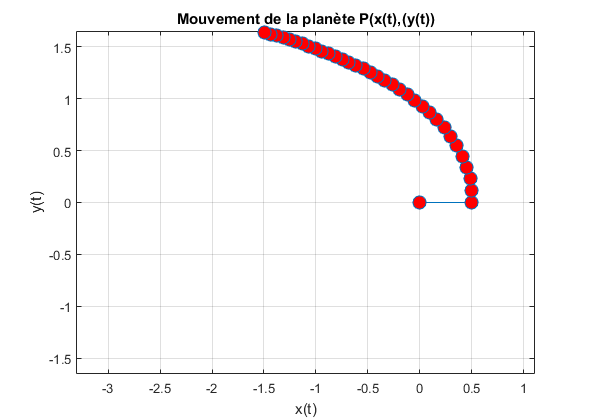
\includegraphics[width=10cm]{fig_euler1}
\centering
\caption{Mouvement de l'astre P avec la méthode d'Euler ($h=0.01$; durée=$2ua$)}
\end{figure}
\\On observe que l'astre dévit de son orbite rapidement et ne le rejoindra plus jamais. On pourrait penser corriger ça en réduisant la vitesse initiale $y'(0)$, en se disant qu'il est normal qu'un astre soit ejecté de son orbite s'il a trop de vitesse. On tente le coup avec $y'(0)=3$ soit une vitesse 4 fois plus faible et obtenons la figure 3:
\begin{figure}[h]
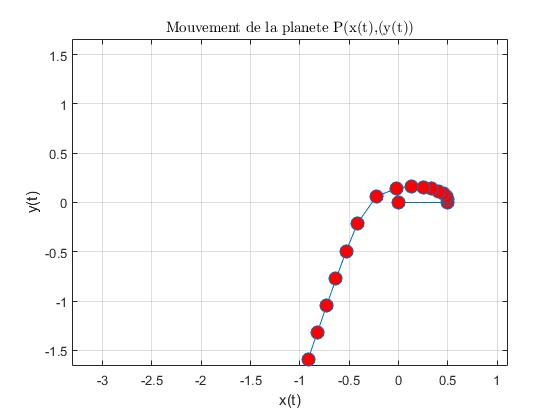
\includegraphics[width=10cm]{fig_euler_vy3}
\centering
\caption{Mouvement de l'astre P avec la méthode d'Euler $(y'(0)=3)$ et ($h=0.01$; durée=$2ua$)}
\end{figure}
\\On voit que cela ne fonctionne pas peu importe la vitesse initialle choisie, on en déduit que ce n'est pas un problème de données erronées. On pourrait modifier la position initiale (sans succès évidemment), mais si l'on commence à trop changer les données de l'enoncé, nous perdons de vue l'objectif de départ.\\
Une donnée sur laquelle on pourrait influer serait celle du pas temporel $h$, en se disant que notre analyse est incorrecte car trop peu précise. Nous prenons donc $h=0.001 ua$ (soit une valeur 10 fois plus petite) et obtenons la figure 4 :
\begin{figure}[h]
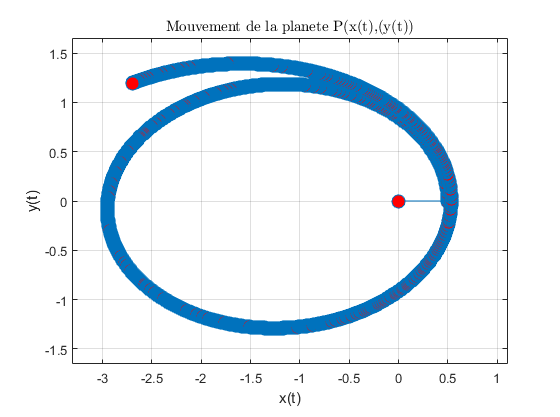
\includegraphics[width=10cm]{fig_euler_h0p001}
\centering
\caption{Mouvement de l'astre P avec la méthode d'Euler ($h=0.001 ua$ et durée=$3ua$)}
\end{figure}
\\ En affichant le mouvement de la planète P sur une durée de $3ua$, nous parvenons à obtenir un tracé plus elliptique mais qui finit par diverger au bout d'un moment. \\
Après toutes les modifications que nous avons effectuées, nous ne sommes pas parvenus à obtenir le tracé elliptique souhaité. Nous en déduisons que la méthode d'Euler, telle quelle, est trop imprécise.
\clearpage

\subsubsection{Runge-Kutta 4}
Nous appelons dans notre \textit{main} (cf. annexe) la fonction \textit{fct\_RK4\_2D\_kepler.m} avec les données de l'énoncé et obtenons la figure 5 suivante :
\begin{figure}[h]
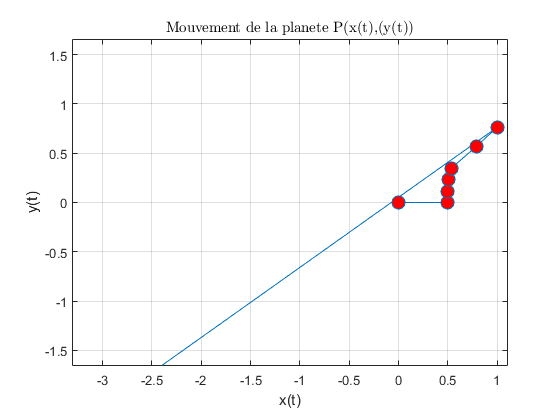
\includegraphics[width=8cm]{fig_rk4_1}
\centering
\caption{Mouvement de l'astre P avec la méthode de Runge-Kutta 4 ($h=0.01$; durée=$2ua$)}
\end{figure}
\\On remarque de suite l'instabilité de l'analyse proposée par cette méthode. On suppose que cette instabilité est causée par des variations trop grandes de valeurs, et proposons donc de prendre un pas $h=0.001$ pour tenter de contourner ce problème. Nous obtenons la figure 6 suivante:
\begin{figure}[h]
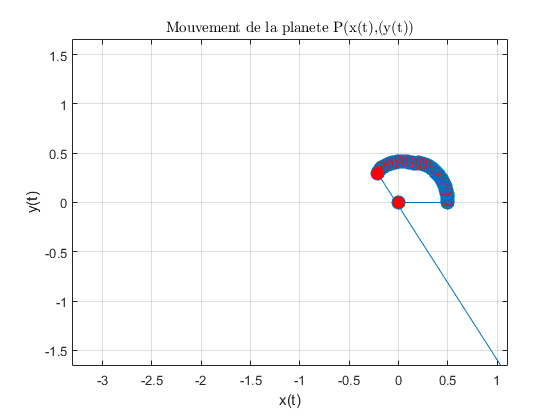
\includegraphics[width=8cm]{fig_rk4_2}
\centering
\caption{Mouvement de l'astre P avec la méthode de Runge-Kutta 4 ($h=0.001$; durée=$2ua$)}
\end{figure}
\\On remarque que l'analyse reste stable plus longtemps, cependant elle diverge au bout d'un certain temps. Nous en déduisons qu'il ne s'agit pas d'une bonne méthode d'analyse pour ce problème. \\
Cependant on remarque, comme avec la méthode d'Euler, qu'influer sur le pas temporel $h$ permet d'améliorer la qualité de l'analyse. C'est pour cela que nous allons analyser ce problème avec la méthode d'Euler-Richardson dans la prochaine partie.
\clearpage
\subsubsection{Euler-Richardson}
Nous appelons dans notre \textit{main} (cf. annexe) la fonction \textit{fct\_Euler\_Richardson.m} avec les données de l'énoncé et obtenons la figure 7 suivante :
\begin{figure}[h]
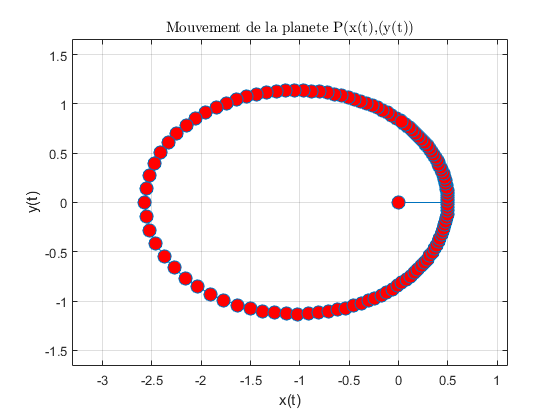
\includegraphics[width=10cm]{fig_euler_rich_1}
\centering
\caption{Mouvement de l'astre P avec Euler-Richardson (durée=$2ua$; $\varepsilon_{seuil}=0.01$)}
\end{figure}
\\On remarque de suite la précision de l'analyse et obtenons bien une ellipse comme attendu. On peut par ailleurs approximer la valeur de la période du mouvement elliptique $T_{période} \approx 2ua$. Par précaution, nous vérifions ce résultat pour une durée=$20 ua$ et obtenons la figure 8 suivante :
\begin{figure}[h]
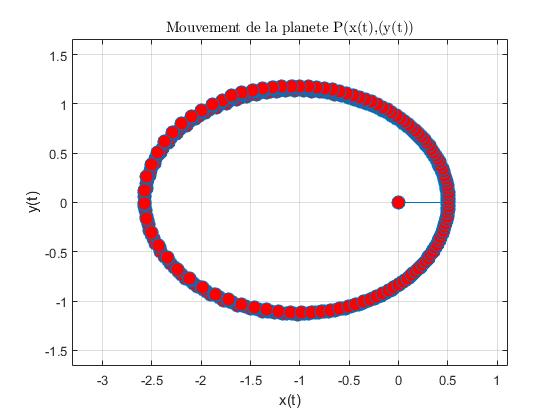
\includegraphics[width=10cm]{fig_euler_rich_2}
\centering
\caption{Mouvement de l'astre P avec Euler-Richardson (durée=$20ua$; $\varepsilon_{seuil}=0.01$)}
\end{figure}
\\ Même après plus de 10 périodes $T_{période}$, nous avons une analyse stable avec une valeur de seuil $\varepsilon_{seuil}=0.01$.
\\\\Un autre point à noter est le nombre de points nécessaires au tracé de l'analyse. Avec la méthode d'Euler, pour avoir un tracé un semblant correct sur $2ua$ nous avions besoin de plus de $10 000$ points, alors qu'avec cette méthode de pas adaptif (et avec $\varepsilon_{seuil}=0.01$), nous n'avons besion que de 140 points. On réduit considérablement le temps de d'exécution du programme.
\\\\ Nous allons maintenant essayer d'afficher le résultat de la figure 7 ($h=0.01$, durée=$2ua$) avec des seuils d'erreur $\varepsilon_{seuil}$ différentes:
\begin{figure}[h]
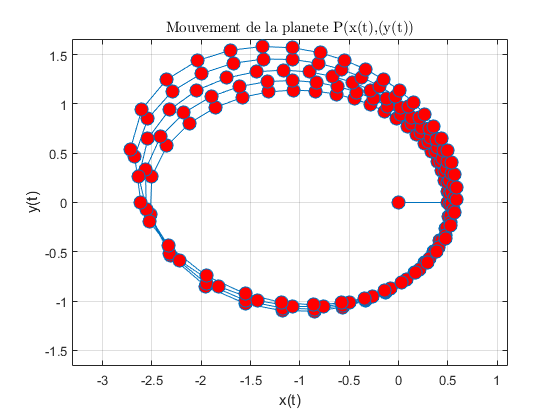
\includegraphics[width=10cm]{fig_euler_rich_3}
\centering
\caption{Mouvement de l'astre P avec Euler-Richardson (durée=$20ua$; $\varepsilon_{seuil}=0.1$)}
\end{figure}
\\ On remarque de suite la divergence qui se crée si on prend $\varepsilon_{seuil} = 0.1$. Ce qui est un résultat attendu.
\begin{figure}[h]
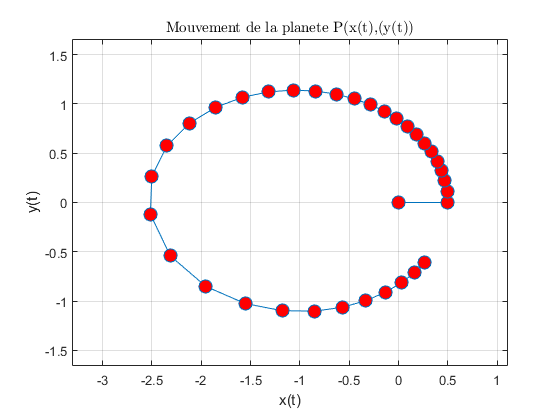
\includegraphics[width=10cm]{fig_euler_rich_4}
\centering
\caption{Mouvement de l'astre P avec Euler-Richardson (durée=$2ua$; $\varepsilon_{seuil}=0.1$)}
\end{figure}
\\ On remarque aussi qu'avec un seuil d'erreur plus important $\varepsilon_{seuil}=0.1$, l'astre P semble parcourir moins de distance (même pas une ellipse complète) qu'avec $\varepsilon_{seuil}=0.01$ (cf. figure 7). Il faut garder en tête que dans cette analyse, le temps est discrétisé et est incrémenté à chaque boucle $t = [t, t(i)+h];$ avec un pas adaptatif $h = 0.9h\times\sqrt{\varepsilon_{seuil}/\varepsilon_2}$ qui augmente plus $\varepsilon_{seuil}$ est grand.
\\\\ Essayons maintenant avec $\varepsilon_{seuil}=0.001$ sur une durée de $2 ua$, nous avons la figure 11 suivante:
\begin{figure}[h]
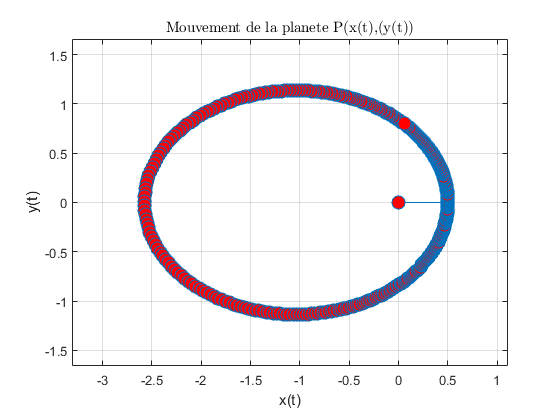
\includegraphics[width=10cm]{fig_euler_rich_5}
\centering
\caption{Mouvement de l'astre P avec Euler-Richardson (durée=$2ua$; $\varepsilon_{seuil}=0.001$)}
\end{figure}
\\On retrouve un résultat semblable à la figure 7 ($\varepsilon_{seuil}=0.01$) avec un nombre de points $n=438$. On aurait pu s'attendre à un nombre de points plus important si l'on pensait qu'avoir une précision $\varepsilon_{seuil}$ 10 fois plus fine impliquerait la création de 10 fois plus de points. On va donc visualiser l'évolution du nombre $n$ de points par rapport à la valeur de $\varepsilon_{seuil}$ sur une durée de $2ua$:
\begin{figure}[h]
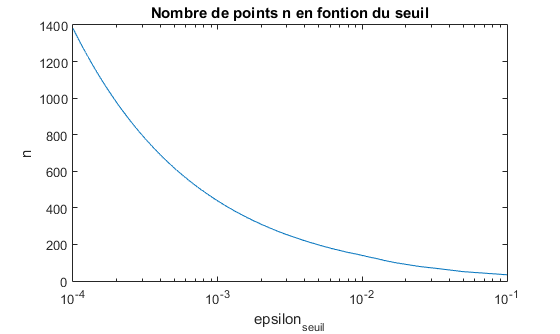
\includegraphics[width=10cm]{fig_euler_rich_6}
\centering
\caption{Evolution du nombre de points $n$ en fonction de $\varepsilon_{seuil}$ (durée=$2ua$)}
\end{figure}
\\ On remarque que la méthode d'Euler-Richardson nous permet d'accéder à des précisions très élevées ($\varepsilon_{seuil}=10^{-4}$) sans pour autant augmenter drastiquement le nombre de points $n$ et donc de calculs à effectuer. On notera cependant que la courbe semble suivre une loi qui ressemble à une loi inverse, et que si l'on souhaite des précisions encore plus fines ($10^{-8}$ par exemple) on aurait alors un nombre de points $n$ qui augmenterait drastiquement et on perdrait l'intérêt de cette méthode.



\clearpage
\section{Double pendule non-amorti}

\subsection{Introduction}

More text.

\subsection{Méthode}

More text.

\subsection{Résultats}

More text.

\clearpage
\section{Annexe}
\subsection{Mouvement Keplérien - fonction \textit{main}}
\lstinputlisting{TP_EDO_Ex6.m}


\end{document}
